\documentclass[usenames,dvipsnames,xcolor=table]{beamer}
\usepackage{subfiles}
\mode<presentation> {

% The Beamer class comes with a number of default slide themes
% which change the colors and layouts of slides. Below this is a list
% of all the themes, uncomment each in turn to see what they look like.

%\usetheme{default}
%\usetheme{AnnArbor}
%\usetheme{Antibes}
%\usetheme{Bergen}
%\usetheme{Berkeley}
\usetheme{Berlin}
%\usetheme{Boadilla}
%\usetheme{CambridgeUS}
%\usetheme{Copenhagen}
%\usetheme{Darmstadt}
%\usetheme{Dresden}
%\usetheme{Frankfurt}
%\usetheme{Goettingen}
%\usetheme{Hannover}
%\usetheme{Ilmenau}
%\usetheme{JuanLesPins}
%\usetheme{Luebeck}
%\usetheme{Madrid}
%\usetheme{CambridgeUS}
%\usetheme{Malmoe}
%\usetheme{Marburg}
%\usetheme{Montpellier}
%\usetheme{PaloAlto}
%\usetheme{Pittsburgh}
%\usetheme{Rochester}
%\usetheme{Singapore}
%\usetheme{Szeged}
%\usetheme{Warsaw}

% As well as themes, the Beamer class has a number of color themes
% for any slide theme. Uncomment each of these in turn to see how it
% changes the colors of your current slide theme.

%\usecolortheme{albatross}
%\usecolortheme{beaver}
%\usecolortheme{beetle}
%\usecolortheme{crane}
%\usecolortheme{dolphin}
%\usecolortheme{dove}
%\usecolortheme{fly}
%\usecolortheme{lily}
%\usecolortheme{orchid}
%\usecolortheme{rose}
%\usecolortheme{seagull}
%\usecolortheme{seahorse}
%\usecolortheme{whale}
%\usecolortheme{wolverine}

%\setbeamertemplate{footline} % To remove the footer line in all slides uncomment this line
%\setbeamertemplate{footline}[page number] % To replace the footer line in all slides with a simple slide count uncomment this line

%\setbeamertemplate{navigation symbols}{} % To remove the navigation symbols from the bottom of all slides uncomment this line
}

\usepackage[T1]{fontenc}
\usepackage[french]{babel}
\usepackage{csquotes}
\usepackage{verbatimbox}

\usepackage{graphicx}
\usepackage{amsmath}
\usepackage{amssymb}  % assumes amsmath package installed
\usepackage{amsfonts}
\usepackage{amsthm}

\DeclareSymbolFontAlphabet{\amsmathbb}{AMSb}%

\usepackage{nicefrac}
\usepackage{tikz}
\usepackage{sidecap}
%\IfFileExists{microtype.sty}{\usepackage{microtype}}{}

\usepackage{placeins}

\usefonttheme[onlymath]{serif}

\usepackage{relsize}
\usepackage{color}

\usepackage{newCommands}

\def\reff{\text{ref}}
\let\epsilon\varepsilon
\let\emptyset\varnothing


\graphicspath{{./}{./img/}{./img/pdf_tex/}}

\usepackage{makecell}

%\usepackage{enumitem}
\usepackage{pifont}

\usepackage{lmodern}
%\usepackage{paralist}
\usepackage{enumerate}
\usepackage{varwidth} 
\usepackage{framed,color}
\definecolor{shadecolor}{rgb}{0.1, 0.6,0.1} 
\def\floatpagefraction{.8}

\beamertemplatenavigationsymbolsempty

\renewcommand{\circled}[1]{\tikz[baseline=(char.base)]{\node[shape=circle,draw,innersep=1pt] (char) {#1};}} 

%\newcommand{\results}[1]{{\small \textit{\textquote{#1}} }}
\newcommand{\results}[1]{{\small \hspace{20pt}\textit{- #1 -} }}
\newcommand{\loc}[1]{\hspace{20pt}{\small #1}}
\newcommand{\CC}{C\nolinebreak\hspace{-.05em}\raisebox{.4ex}{\tiny\bf+}\nolinebreak\hspace{-.10em}\raisebox{.4ex}{\tiny\bf +}}\def\CC{{C\nolinebreak[4]\hspace{-.05em}\raisebox{.4ex}{\tiny\bf ++}}}

\newcommand{\tblue}[1]{\textcolor{blue}{#1}}
\newcommand{\tfblue}[1]{\textcolor{blue}{\textbf{#1}}}

\date{\today} % Date, can be changed to a custom date

\begin{document}
\begin{frame}
\begin{center}
    \textcolor{blue}{
    \textbf{
    {\Large
    Robotics from perspectives\\[4pt]
    }}
    }
    \rule{.9\linewidth}{2pt}\\[4pt]
    Philipp Schlehuber-Caissier \\
    Post-Doc, LRDE, Epita\\[6pt]
    \rule{.9\linewidth}{2pt}\\[4pt]
 	15 janvier 2019\\
    Orientation week
    
\end{center}
\end{frame}

%%%%%%%%%%%%%%%%%%%%%%%%%%%%%%%%%%%%%%%%%%%%%%%%%%%%%%%%

\section{Table of Contents}

\begin{frame}{Overview}
    \begin{itemize}
        \item The historical perspective
        \item The control theoretic perspective
        \item The industrial perspective
        \item My perspective
    \end{itemize}
\end{frame}

\section{The}

\section{The industrial perspective}
\begin{frame}{The industrial perspective}
\begin{center}
    
\end{center}
\end{frame}

\begin{frame}
    \frametitle{Curriculum Vit\ae ~ 1/2}
    \bgroup
    \def\arraystretch{2.5}
    %\begin{center}
    \begin{tabular}{c|l}
         2007 & \makecell[l]{\tblue{Abitur (Bac) avec focalisation math\'ematique/physique} \\ \loc{Christoph Scheiner Gymnasium, Ingolstadt, Allemagne} \\ \results{Mention tr\`es bien} }  \\ \hline
         2007-11 & \makecell[l]{\tblue{Formation en alternance g\'enie m\'ecanique et m\'ecanicien} \\ \loc{TH N\"urnberg et Schaeffler AG, N\"uremberg, Allemagne} \\ \results{Mention tr\`es bien, 2$^e$/150} } \\ \hline
         2011-13 & \makecell[l]{\tblue{Ing\'enieur R{\&}D chez Schaeffler AG} \\ \loc{Simulation et optimisation num\'erique} \\ \loc{Schaeffler AG, Herzogenaurach, Allemagne}} \\ \hline
         2013-2015 & \makecell[l]{\tblue{Master syst\`emes avanc\'es et robotique} \\ \loc{Univ. Pierre et Marie Curie, Paris, France} \\ \results{Mention tr\`es bien, 2$^e$/40} }
    \end{tabular}
    %\end{center}
    \egroup
\end{frame}

%%%%%%%%%%%%%%%%%%%%%%%%%%%%%%%%%%%%%%%%%%%%%%%%%%%%%%%%

\begin{frame}
    \frametitle{Curriculum Vit\ae ~ 2/2}
    \begin{minipage}{\linewidth}
    \bgroup
    \def\arraystretch{2.5}
    \begin{center}
    \begin{tabular}{c|l}
        2015-18 & \makecell[l]{\tblue{Th\`ese en Robotique} \\ \loc{\textit{Contributions to robotic control design}}\\\loc{\textit{under formal stability and safety constraints}} \\ 
        \loc{Vincent PADOIS et Nicolas PERRIN}\\
        \loc{ISIR-SORBONNE UNIVERSIT\'E, Paris, France}} \\ \hline
        2018-19 & \makecell[l]{\tblue{Attach\'e temporaire d'enseignement et de recherche} \\ \loc{Enseignements divers en informatique, \'electronique}\\\loc{et m\'echanique} \\ \loc{ISIR-SORBONNE UNIVERSIT\'E, Paris, France} }
    \end{tabular}
    \end{center}
    \egroup
    \end{minipage}
    \vspace*{\fill}
\end{frame}

%%%%%%%%%%%%%%%%%%%%%%%%%%%%%%%%%%%%%%%%%%%%%%%%%%%%%%%%

\section{Enseignement}

\begin{frame}
\frametitle{Enseignement}

\begin{columns}
\begin{column}{0.49\linewidth}
\bgroup
\def\arraystretch{1.5}
\begin{tabular}{|c|c|}
    \hline
     2015-18 & Moniteur - 3x64h  \\ \hline
     2018-19 & ATER - 192h \\ \hline
\end{tabular}
\egroup
\vspace{10pt}
\begin{itemize}
    \item 24h~CM,~130h~TD,~167h~TP
    \item 80h~Projet
    \item 335h Licence
    \item 66h Master
\end{itemize}

\end{column}

\begin{column}{0.02\linewidth}
\end{column}

\begin{column}{0.49\linewidth}
{\centering Liste des UEs incomplets}
\begin{itemize}
    \item Programmation scientifique et simulation physique (Python-M1)
    \item Programmation en langage objet (\CC-M1)
    \item Programmation pour le calcul scientifique (Fortran-L2)
    \item Projet Romarin (L2)
\end{itemize}
\end{column}
\end{columns}

\end{frame}
%%%%%%%%%%%%%%%%%%%%%%%%%%%%%%%%%%%%%%%%%%%%%%%%%%%%%%%%

\begin{frame}
    \frametitle{Enseignement - Projet Romarin}
    \vspace{-10pt}
    \begin{center}
    \textbf{\textbullet Apprentissage par projet \hspace{20pt} \textbullet Projet pluridisciplinaire} \\
    \bigskip
    
    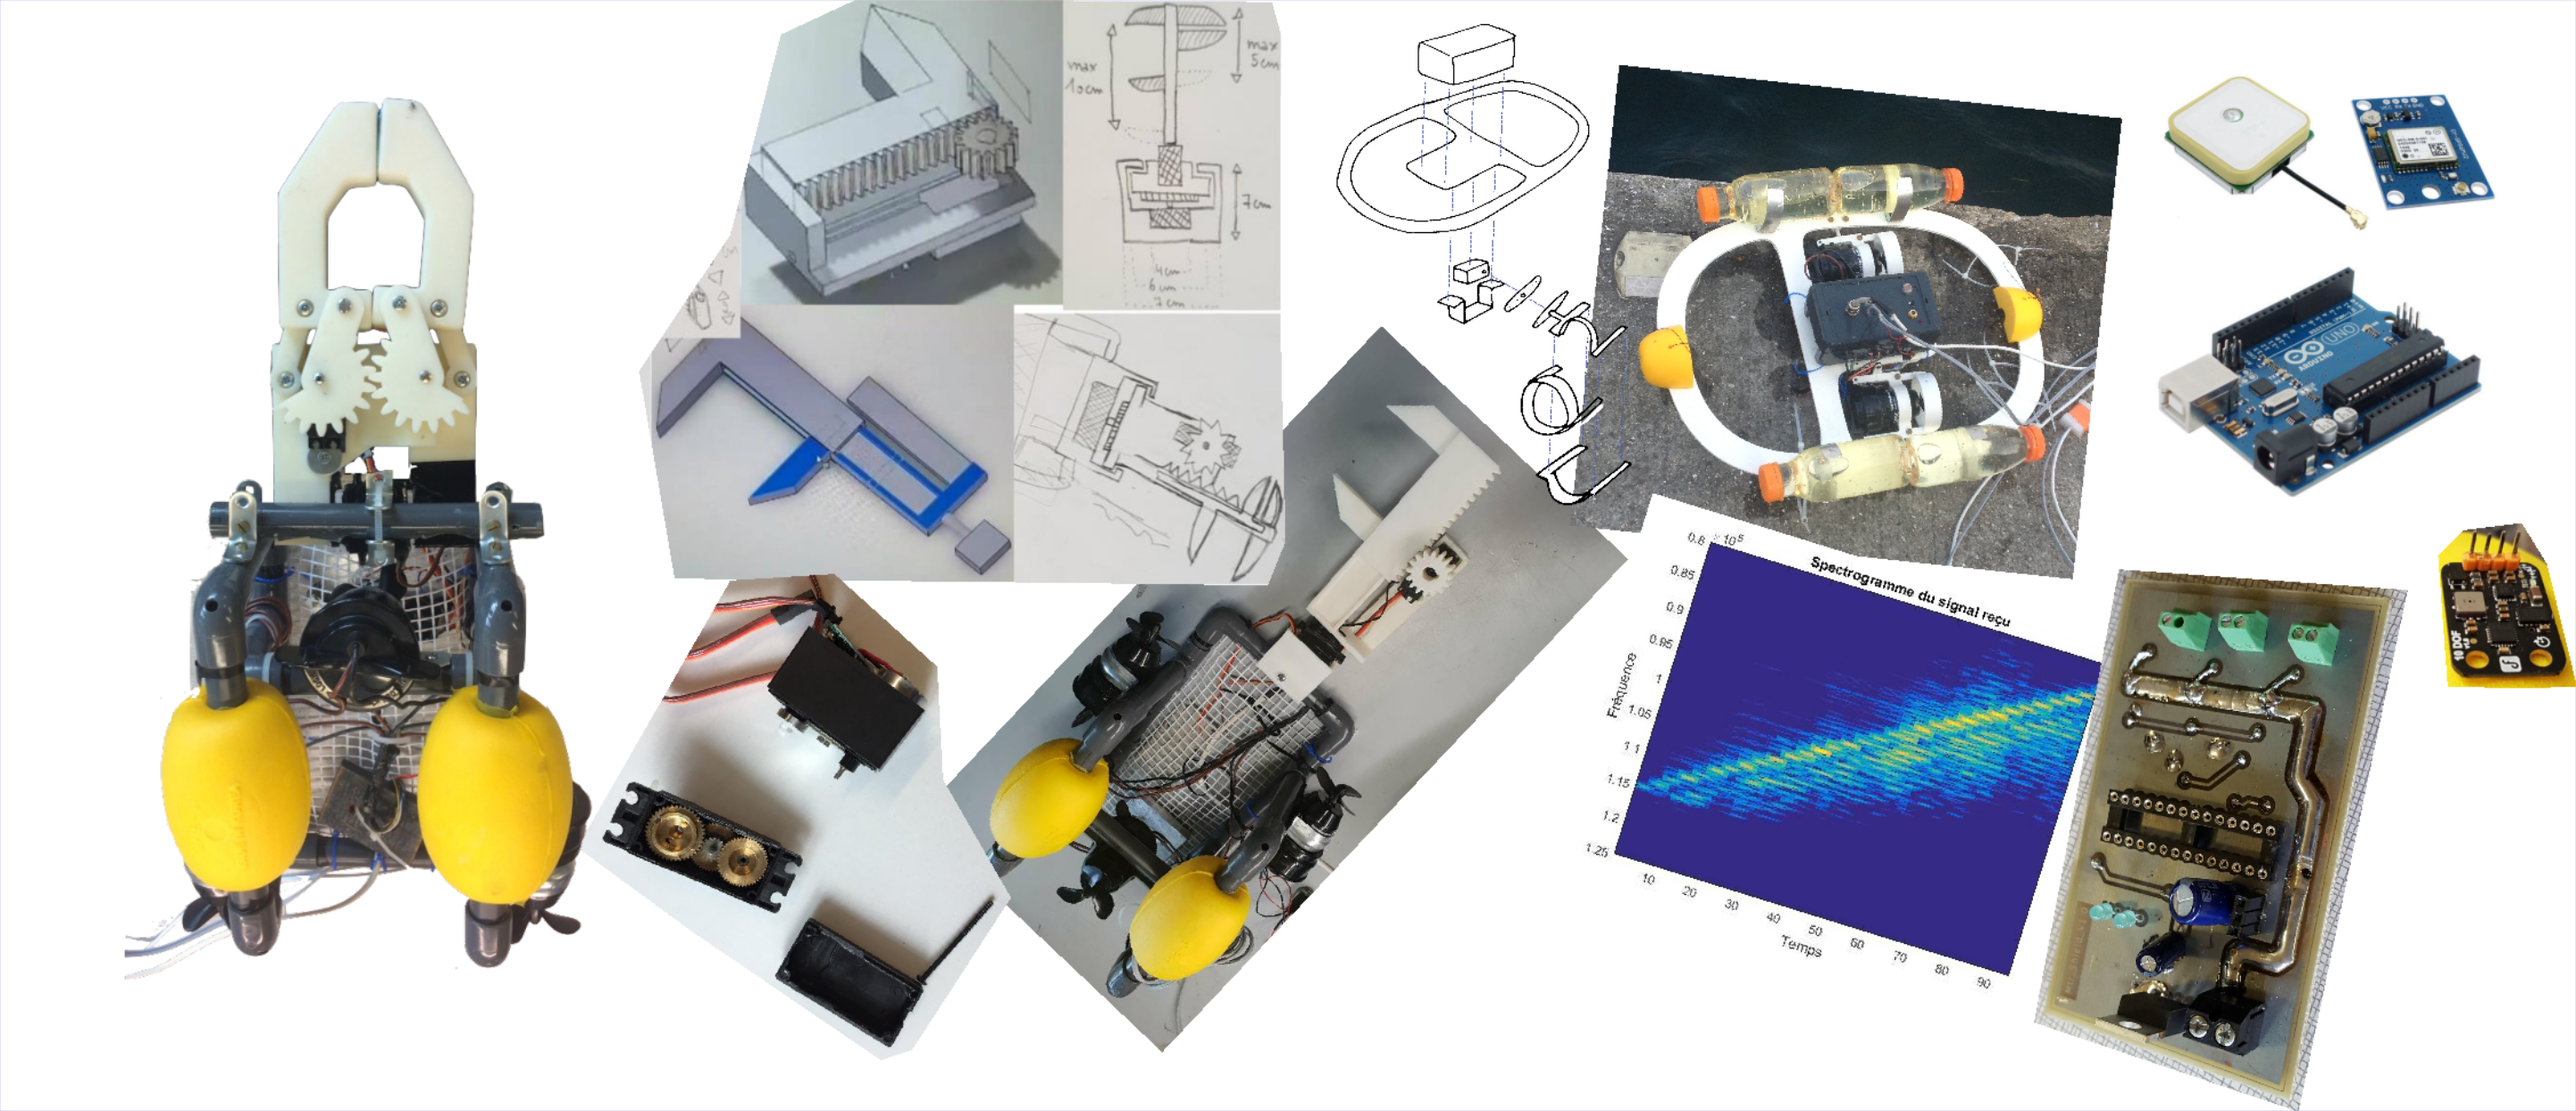
\includegraphics[width=1.\linewidth]{romarin4.png}
    \end{center}
   
    
\end{frame}

%%%%%%%%%%%%%%%%%%%%%%%%%%%%%%%%%%%%%%%%%%%%%%%%%%%%%%%%

\section{Recherche}

\begin{frame}
    \frametitle{Th\'ematiques de recherche}
    \vspace{-6pt}
    \begin{center}
        {\large \textbf{Obtenir des garanties formelles pour la contr\^ole}}
    \end{center}
    
    \begin{center}
    \bgroup
    \def\arraystretch{2.5}
    \begin{tabular}{c|c}
        \textbf{Objectif} & \textbf{M\'ethode} \\ \hline
         \only<1>{\makecell{Synth\`ese automatique\\de loi de contr\^ole}}
         \only<2>{\tfblue{\makecell{Synth\`ese automatique\\de loi de contr\^ole}}} & \only<1>{\makecell{Robot + T\^ache\\$\mapsto$ Automates temporis\'es}} \only<2>{\tfblue{\makecell{Robot + T\^ache\\$\mapsto$ Automates temporis\'es}}} \\ \hline
         Stabilit\'e des syst\`emes & \makecell{Contr\^ole optimal et\\optimisation convexe} \\ \hline
         \only<1>{\makecell{Apprentissage\\par d\'emonstration}}
         \only<2>{\tfblue{ \makecell{Apprentissage\\par d\'emonstration} } }& 
         \only<1>{\makecell{Couplage des diff\'eomorphisme \\ et de \textit{machine learning} }}
         \only<2>{\tfblue{\makecell{Couplage des diff\'omorphisme \\ et de \textit{machine learning} }}}
    \end{tabular}
    \egroup
    \end{center}
\end{frame}

%%%%%%%%%%%%%%%%%%%%%%%%%%%%%%%%%%%%%%%%%%%%%%%%%%%%%%%%

\begin{frame}
    \frametitle{Th\'ematiques de recherche - Synth\`ese}
    \vspace{-30pt}
    \begin{center}
        \mbox{\textbf{\textbullet~Abstraction du syst\`eme en TA \hspace{2pt} \textbullet~Synth\`ese $\Leftrightarrow$ Atteignabilit\'e}} \\
	\vspace{15pt}
    %{\centering \textbullet~Abstraction du syst\`eme en TA \hspace{10pt} \textbullet~Synth\`ese $\Leftrightarrow$ atteignabilit\'e}
 		\def\svgwidth{\linewidth}
		{\relscale{.7}
		\input{./img/pdf_tex/tempAutIntro4_fr.pdf_tex}
		}
	\end{center}    
    
\end{frame}

%%%%%%%%%%%%%%%%%%%%%%%%%%%%%%%%%%%%%%%%%%%%%%%%%%%%%%%%

\begin{frame}
    \frametitle{Th\'ematiques de recherche - Commande et apprentissage}
    \vspace{-10pt}
    \begin{center}
        \hspace{-30pt}\textbf{\textbullet~Apprendre des mouvements \hspace{25pt} \textbullet~Assurer la stabilit\'e} \\ 
        \vspace{15pt}
        \def\svgwidth{0.99\linewidth}
		{\relscale{.7}
		\input{./img/pdf_tex/diffeoIntro1_2.pdf_tex}
		}
    \end{center}
    %{\centering \textbullet~Apprendre des mouvements \hspace{10pt} \textbullet~Assurer la stabilit\'e}
\end{frame}

%%%%%%%%%%%%%%%%%%%%%%%%%%%%%%%%%%%%%%%%%%%%%%%%%%%%%%%%

\begin{frame}
    \frametitle{Th\'ematiques de recherche - Perspective}
	\vspace{-10pt}
    \begin{center}
	    \textbf{Synth\`ese \textit{formelle} des strategi\`es }    
	\vspace{0pt}
    %\begin{center}
    %\begin{minipage}{0.8\linewidth}
    \begin{columns}
    \begin{column}{0.5\linewidth}
    \begin{itemize}
        \item Lien avec l'ANR TickTac
        \item Passage \'a l'\'echelle
    \end{itemize}
    \end{column}
    \begin{column}{0.5\linewidth}
    \begin{itemize}
    	\item Appliquabilit\'e de la verification \`a la robotique
    	\item Couplage TA et LTL    
    \end{itemize}
    \end{column}
    \end{columns}    
    %\end{minipage}
    %\end{center}
    
    \vspace{10pt}
    \def\svgwidth{0.7\linewidth}
	{\relscale{1.}
	\input{./img/pdf_tex/perspective.pdf_tex}
	}    
    \end{center}
\end{frame}

%%%%%%%%%%%%%%%%%%%%%%%%%%%%%%%%%%%%%%%%%%%%%%%%%%%%%%%%

\section{R\'esum\'e}

\begin{frame}
    \frametitle{R\'esum\'e}
    
    \begin{itemize}
        \item Profil pluridisciplinaire
        %\item Exp\'eriences dans l'industrie
        %\item Exp\'eriences dans l'enseigment
	    %\item Exp\'erience dans les m\'ethodes formelles, en particulier les automates temporis\'es
	    %\item Exp\'eriences en th\'eorie de la commande et optimisation
	    
	    \item Exp\'eriences
	    \begin{itemize}
	        \item[\ding{212}] dans l'industrie
	        \item[\ding{212}] dans l'enseignement
	        \item[\ding{212}] dans les m\'ethodes formelles,\\en particulier les automates temporis\'es
	        \item[\ding{212}] en th\'eorie de la commande et optimisation
	    \end{itemize}
	    \item M\^aitrise de Python, Cuda et \CC
    \end{itemize}
	\begin{center}
		\visible<2>{ \textcolor{blue}{{\Large \textbf{Merci pour votre attention!} } }	}
	\end{center}
    
\end{frame}

%%%%%%%%%%%%%%%%%%%%%%%%%%%%%%%%%%%%%%%%%%%%%%%%%%%%%%%%

\end{document}

